\chapter[从工具到助手]{从工具到助手：现实世界中的应用}
\label{sec:assist}

\begin{learningbox}
本章将介绍智能体语言模型如何在现实世界的不同领域中部署为实用助手。
具体而言，学完本章后，你将能够：
\begin{itemize}[leftmargin=*, nosep]
    \item 描述助手如何超越问答，进行规划、检索信息、调用工具，并随着时间的推移{\em 调整自身行为}。
    \item 比较{\em 购物、医疗、航空、科学研究和编程}等领域中的助手架构。
    \item 解释为什么高风险领域会对{\em 安全性、透明性和法规合规}提出更严格的要求，以及智能体设计如何回应这些要求。
    \item 批判性地评估助手行为，并思考在对社会具有重要影响的场景中部署智能体系统所涉及的{\em 伦理}问题。
\end{itemize}
\end{learningbox}

\section{作为助手的智能体大语言模型}
大语言模型（large language model，LLM）已经从文本生成器发展为主动提供协助的助手。它们将推理、检索和工具使用结合起来，在现实世界中采取行动。助手是智能体大语言模型（agentic LLM）的实际软件形态：这类系统能够交互、规划，并从反馈中学习。助手让推理与现实相接，使语言模型成为能够在世界中协作行动的参与者。

助手将感知、推理与行动联系起来。借助应用程序接口（application programming interface，API）和外部工具，它能够开展对话、执行任务，并适应特定情境。这类系统不仅为用户提供支持，还会产生有价值的人类与人工智能交互数据；我们可以利用这些数据继续开展研究与开发，并训练下一代模型。

本章回顾主要的助手类型。我们首先介绍对话系统，以及它们如何向多模态、能够使用工具的交互界面演进。接下来讨论医疗、金融和交易等领域的专用助手。最后介绍用于推理与发现的科学助手。

\section{对话助手}

第一个应用领域是一般对话场景，例如通过记录会议纪要、担任会议主持人或一般行政助理来协助会议。

在这类应用中，大语言模型的基本作用，是让人机交互更加自然、顺畅 \citep{neszlenyi2024assistantgpt,oluwagbade2024conversational}。例如，AssistantGPT 系统 \citep{neszlenyi2024assistantgpt} 是一款通用行政助手，面向教育机构或企业环境部署。它还支持 Teams 和 Slack 等远程办公环境。AssistantGPT 支持多种操作，包括网页搜索、通过 OpenAPI 与 API 交互、语音对话，以及通过 shell 执行命令。该系统由一个大语言模型组成，并可访问规划器、记忆等多种工具（见图~\ref{fig:assist}）。

\begin{figure}
  \begin{center}
    % 按 figures/assist.png 的六条工具/记忆/规划关系及用户输入关系重绘。
\resizebox{10.2cm}{!}{%
\begin{tikzpicture}[x=1cm,y=1cm,
  every node/.style={font=\normalsize,align=center},
  unit/.style={draw=black!50,line width=.65pt,rounded corners=1pt,
    minimum height=.82cm,minimum width=1.8cm,fill=cyan!18},
  edge/.style={-{Stealth[length=2.7mm,width=1.9mm]},line width=.8pt,draw=black!75},
  relation/.style={fill=white,inner sep=2pt,font=\small}]
  \node[unit,fill=yellow!35,minimum width=2.7cm] (ch13request) at (4.8,5.7) {用户请求};
  \node[unit,fill=green!17,minimum width=1.7cm] (ch13agent) at (4.8,2.6) {智能体};
  \node[unit] (ch13tools) at (1.0,0) {工具};
  \node[unit] (ch13memory) at (4.8,0) {记忆};
  \node[unit,minimum width=2.0cm] (ch13plan) at (9.2,0) {规划};
  \draw[edge] (ch13request.south) -- node[relation,right,pos=.54] {与之交互} (ch13agent.north);
  \draw[edge] (ch13agent.south west) -- node[relation,above left,pos=.55] {使用} (ch13tools.north east);
  \draw[edge] (ch13tools.west) .. controls (-1.35,1.0) and (-.8,2.0) .. (ch13agent.west);
  \node[relation] at (-.05,1.35) {执行};
  \draw[edge] (ch13agent.south west) .. controls (3.45,1.55) and (3.6,.9) .. (ch13memory.north west);
  \node[relation] at (4.25,1.35) {存储};
  \draw[edge] (ch13memory.north) .. controls (5.17,1.1) and (5.17,1.65) .. (ch13agent.south);
  \node[relation] at (5.65,1.35) {检索};
  \draw[edge] (ch13agent.south east) -- node[relation,above right,pos=.62] {规划} (ch13plan.north west);
  \draw[edge] (ch13plan.north) .. controls (8.65,1.85) and (7.2,2.28) .. (ch13agent.east);
  \node[relation] at (9.5,1.35) {更新};
  % 原图中的用户图标与其标签。
  \draw[draw=black!55,line width=.7pt] (7.65,6.42) circle (.18);
  \draw[draw=black!55,line width=.7pt] (7.65,6.24) -- (7.65,5.55)
    (7.32,6.02) -- (7.98,6.02)
    (7.65,5.55) -- (7.31,5.15)
    (7.65,5.55) -- (7.99,5.15);
  \node[font=\small] at (7.65,4.93) {用户};
\end{tikzpicture}%
}

    \caption{AssistGPT 系统架构 \citep{neszlenyi2024assistantgpt}}\label{fig:assist}
  \end{center}
\end{figure}

已有研究表明，这类对话与会议助手能够改善敏捷软件开发团队的会议 \citep{cabrero2024exploring}。它们在 Scrum 会议的准备工作和会议期间的即时协助中取得了良好效果，不过，一些测试者认为，大语言模型的介入显得不够自然，也不够灵活。

其他例子包括协作学习课堂中的大语言模型智能体，它们改善了参与者之间的整体协作 \citep{wei2024improving}。另一项研究 \citep{bastola2023llm} 则在一项包含对话助手的协作任务调度实验中，报告了工作效率的提高。

另一类略有不同的助手是思考助手（thinking assistant）。它通过提问而非作答，尝试改善人类在面对艰难决策时的反思性思考 \citep{park2023thinking}。大型大语言模型供应商最近也推出了类似尝试，例如 OpenAI 的 ChatGPT 和 Google 的 Gemini 应用中的{\em 学习模式（Study mode）}。

对话助手大多由常规预训练大语言模型演化而来，有时会针对特定领域进行微调。一些方法采用由多个专用大语言模型组成的方案，让不同模型分别处理不同子任务；另一些方法则为单个大语言模型编排不同的提示序列，使其分别聚焦于不同子任务。

\section{购物助手}

本节考察基于语言的助手如何应用于电子商务领域。我们的目标是突出这一领域中的主要组件、架构选择，以及领域特有的挑战。

\paragraph{购物助手能做什么？}
购物助手是基于大语言模型构建的对话系统，帮助用户完成在线购物任务。它可以帮助用户理解产品需求、比较备选产品、获得商品推荐并完成购买。这类系统通常会在基础大语言模型之外加入领域专用模块，包括检索最新产品信息、通过 API 访问产品目录、集成推荐引擎，以及围绕用户需求、产品属性和约束进行推理，例如使用思维链（chain of thought）。

\paragraph{关键要素}
通用大语言模型并未内置对电子商务概念的充分认识，例如品牌、类别、产品层级与用户购买行为。因此，要构建能力出色的助手，就需要从以下几个方面增强模型：
\begin{itemize}
  \item 检索增强：从外部来源动态获取产品元数据、价格与库存情况。
  \item 工具／API 调用：助手可以调用搜索、筛选与排序工具，与产品数据库交互。
  \item 领域微调或指令微调：使大语言模型适应购物情境，包括品牌相关用语、属性推理与用户意图。
  \item 结构化推理：加入思维链提示或显式推理步骤。这有助于模型比较产品、评估不同因素之间的权衡，例如价格与功能之间的权衡，并与用户偏好保持一致。
\end{itemize}

\paragraph{购物助手的基准测试}
为了研究模型处理购物专属任务的能力，研究者开发了相应的基准测试。例如，{\em 多任务在线购物基准数据集（Multi-task Online Shopping Benchmark dataset，ShopMMLU）}~\citep{jin2024shopping} 定义了 57 项任务，归为四类技能：概念理解、知识推理、用户行为对齐和多语言能力。它采用真实的电子商务数据，包括 Amazon 的产品目录、会话与评论，评估大语言模型处理品牌与型号识别、产品兼容性推理、基于会话的推荐任务和多语言查询等问题的能力。
另一个例子是 LLaSA 系统（large language and E-commerce shopping assistant）\citep{zhang2024llasa}，它使用一个名为 {\em EshopInstruct}、包含 65,000 个样本的指令数据集进行训练。经过购物任务的指令微调后，LLaSA 在 ShopBench 基准测试中取得了优异结果，表明适应性训练能够显著改善模型在这一领域的表现。

\paragraph{实践建议}
构建购物助手时，以下原则十分重要：
\begin{itemize}
  \item 能力出色的助手需要结合自然语言理解与领域推理。它应当理解{\em 价格低于 200 欧元、续航 > 20 h 的降噪耳机}是什么意思，并能够将其转化为产品属性与用户约束。
  \item 领域专用数据很重要：现成的大语言模型虽然能够发挥一定作用，但在购物任务上进行微调或指令微调，可以显著提高表现。LLaSA \citep{zhang2024llasa} 在实践中展示了这一点。
  \item 评估必须反映领域特点。与理解产品属性或生成查询的准确性相比，助手能否与用户行为保持一致、处理多步会话并支持多语言用户更为重要。
  \item 工具与检索的集成至关重要。助手必须充当产品系统的交互接口，而不能仅仅作为一个纯粹的语言模型。这会带来额外的复杂性，包括 API 设计、延迟、数据时效性，以及集成错误的处理。
  \item 考虑伦理与信任问题。在购物场景中，推荐涉及商业利益、隐私与偏见。在将这类系统部署到生产环境之前，应当通过以下问题评估这些方面：{\em 展示了哪些品牌}、{\em 是否正确处理了用户历史记录}，以及{\em 推理过程有多透明}。
\end{itemize}

\paragraph{挑战与开放问题}
尽管近年来取得了进展，购物助手仍面临几个不容小觑的挑战。首先，大语言模型智能体仍然难以处理较长的交互轨迹，包括浏览、细化查询与切换意图。其次，实时更新产品知识，例如新型号、价格变化与库存情况，仍然是一个突出的工程难点。第三，在基于大语言模型的助手中，如何向用户解释和论证推荐理由，例如为什么推荐这一产品而非另一产品，仍缺少充分研究。最后，跨语言行为与多语言产品查询进一步增加了复杂性，因为购物情境跨越不同语言和地区。

\section{飞行运行助手}

基于语言的助手也应用于飞行运行（flight operations）。这一领域已经超越面向消费者的预订服务，进入规划与决策支持环节。

\paragraph{预订与旅行规划}
对话式预订助手是一种相对简单的应用，与上一节的购物助手类似。例如，\citet{manasa2024towards} 提出了一个基于 LLaMa 2 和检索增强生成（retrieval-augmented generation，RAG）的系统，以交互方式帮助用户预订航班。该助手使用航班预订数据进行微调，并通过检索接入最新航班信息。在用户测试中，它在捕捉用户偏好和高效引导预订流程方面获得了较高评价。

请注意，这个应用场景在运行层面仍然相对简单。助手处理的是结构化用户意图，例如{\em 我想在日期 D 从 A 飞往 B}，以及最新产品数据的检索、偏好获取（preference elicitation）和回答生成。它尚未深入涉及动态空中交通约束或安全裕度等问题。

\paragraph{运行决策支持}
在要求更高的场景中，研究者开始提出用于实际飞行运行的大语言模型助手。我们讨论两个例子。

在 \citet{zhou2024flight} 的研究中，到达时隙分配问题，即确定到达飞机应以何种顺序着陆，被表述为一个语言建模任务。作者将调度输入与输出编码为词元，并对大语言模型进行微调，使其生成无冲突的着陆序列。实验表明，即使在传统方法难以奏效的机场，该模型也能降低冲突率和总延误时间。

另一个运行问题是在环境危险条件下进行规划。\citet{tabrizian2024using} 使用思维链，在风害约束下支持航路或飞行计划生成。在这里，助手的任务不再只是{\em 预订航班}，而是必须围绕风、航路、飞机性能等约束进行推理，并提出运行上可行的计划。

\paragraph{主要建议}
这些研究展示了基于大语言模型的智能体系统的几个重要方面：

\begin{itemize}
    \item 工具／后端集成：在运行助手中，大语言模型除了开展对话，还必须与航班数据库、天气数据源、航路规划引擎和时隙分配系统对接。这意味着要实现工具调用、检索流程与决策逻辑。
    \item 约束条件下的推理：这类助手必须处理组合约束或调度约束，生成计划，并应对天气、跑道可用性等实时不确定性。到达时隙分配就是一个很好的例子，其中大语言模型必须对动态排序进行推理。
    \item 领域专用数据与微调：标准预训练大语言模型缺乏关于飞行运行的先验知识。上述系统都针对这一领域进行了微调或专门设计了提示。需要准备适合该领域的任务数据集、提示、预期输出与评估指标。
    \item 从对话智能体到自主规划器：预订助手仍由用户驱动，即用户提问、助手提供帮助；运行助手则越来越多地承担规划角色。助手应当能够处理诸如{\em 这些是约束条件，请提出调度方案或航路}这样的请求。这种变化带来了信任、验证与可解释性问题。
    \item 真实情境中的评估：对运行系统的评估往往不只是考察{\em 助手是否回答了用户}，还要衡量冲突率、延误时间和序列效率等方面。例如，到达时隙分配的大语言模型研究就测量了总延误时间与冲突率。
\end{itemize}

\section{医疗助手}
医疗是大语言模型助手应用最活跃的领域之一 \citep{thirunavukarasu2023large,clusmann2023future,mehandru2024evaluating}。近期研究报告，大语言模型在诊断任务中能够超过受过训练的医生 \citep{goh2024large}，在临床记录生成方面也能够超过人工医疗记录员 \citep{yuan2024continued}。其他评估证实了这些优势，同时也发现了模型在特定临床场景中的系统性弱点 \citep{panagoulias2024evaluating}。

智能体架构正越来越多地用于满足监管、伦理和可用性要求。\citet{sudarshan2024agentic} 提出了一种智能体工作流程，用于生成患者易于理解、符合《21 世纪治愈法案》（21st Century Cures Act）的医疗报告。他们的系统使用反思（reflexion；第~\ref{sec:self-reflection}~节，\citep{shinn2024reflexion}），在向患者发布信息之前，迭代改善报告的清晰度与正确性。

其他研究探索了大语言模型智能体在更广泛临床支持中的用途。\citet{qiu2024llm} 指出了从临床工作流程自动化到多智能体诊断支持等应用，不过，准确性、完整性和幻觉问题仍然令人担忧。\citet{ullah2024challenges} 的一项范围综述（scoping review）强调，训练与微调这类系统时，医疗领域知识与伦理约束不可或缺。

为了缓解常见失效模式，\citet{das2024improved} 提出了一种基于检索的智能体架构，其中大语言模型充当规划器，而不直接生成答案。智能体协调专用工具，从可信医疗来源中检索并综合证据，从而减少幻觉和{\em “迷失在中间”（lost-in-the-middle）}错误。

\paragraph{高风险应用领域}
医疗是高风险应用领域，错误或有偏见的输出可能直接危及患者安全。因此，医疗人工智能系统受到严格监管框架的约束，包括将许多医疗人工智能用途归类为高风险的欧盟《人工智能法案》（EU AI Act）。无论在临床实践中，还是在医疗大语言模型的学术研究中，透明性、公平性和问责性都处于核心地位。
这些关切促使人们更加关注超越事后解释、试图在更深层次理解模型行为的方法。我们将在{\em 机制可解释性（mechanistic interpretability）}一章（第~\ref{chap:mi}~章）回到这一主题，讨论分析和控制模型内部表征的技术。

\paragraph{医学教育}
在医学教育中，智能体系统被用来模拟真实的训练环境。\citet{wei2024medco} 提出了一种多智能体协同助手，支持基于病例的学习与临床推理练习（图~\ref{fig:medco}）。对于医疗检索增强生成的系统性评估，\citet{qiao2024benchmarking} 提供了一项专用基准测试。

\begin{figure}
  \begin{center}
    % 在原图上仅覆盖自然语言文字区域，保留全部图标、面板、对话框边框及数据含义。
\begingroup
\linespread{1}\selectfont
\definecolor{ch13MedPink}{RGB}{247,214,207}
\definecolor{ch13MedGreen}{RGB}{229,240,219}
\definecolor{ch13MedYellow}{RGB}{253,242,208}
\definecolor{ch13MedGray}{RGB}{237,237,237}
\newlength{\chThirteenMedUnit}
\setlength{\chThirteenMedUnit}{\dimexpr\linewidth/1748\relax}
\newcommand{\chThirteenMedBlock}[7]{%
  \fill[#5] (#1,#2) rectangle (#3,#4);
  \node[inner sep=0pt,align=left,
    text width=\dimexpr#3\chThirteenMedUnit-#1\chThirteenMedUnit-12\chThirteenMedUnit\relax,
    font=#6] at ({(#1+#3)/2},{(#2+#4)/2}) {#7};
}
\begin{tikzpicture}[x=\chThirteenMedUnit,y=-\chThirteenMedUnit]
  \node[anchor=north west,inner sep=0pt] at (0,0) {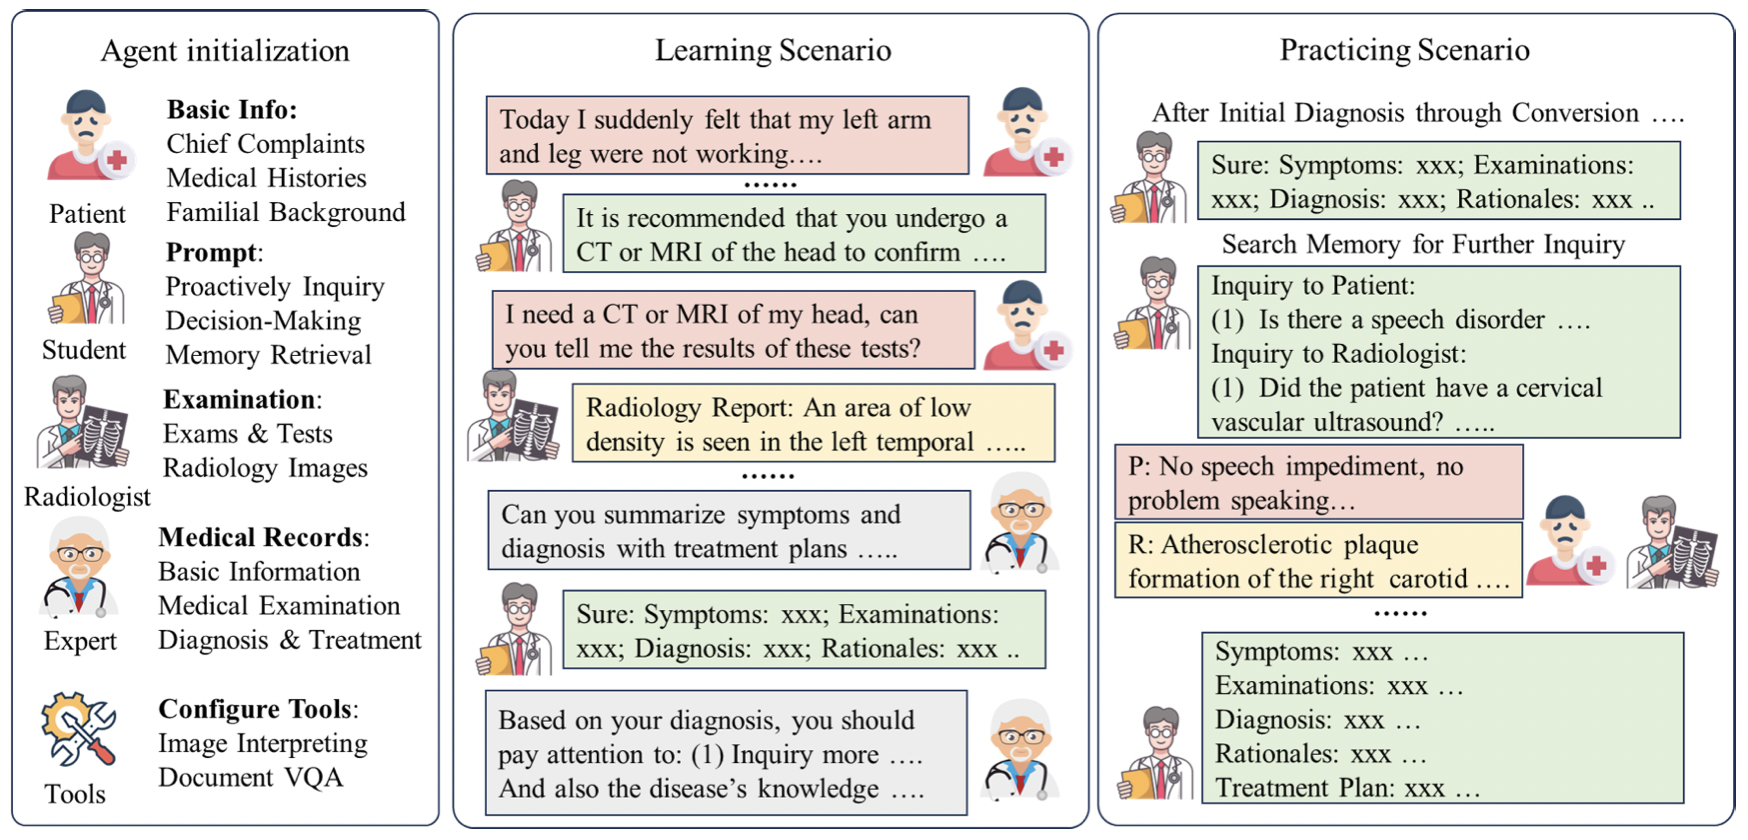
\includegraphics[width=\linewidth]{figures/medco.png}};
  % 智能体初始化面板：原有角色和全部字段。
  \fill[white] (55,28) rectangle (414,75);
  \node[font=\fontsize{9}{11}\selectfont\bfseries] at (234,51) {智能体初始化};
  \chThirteenMedBlock{20}{199}{151}{229}{white}{\fontsize{8.2}{10}\selectfont}{\centering 患者}
  \chThirteenMedBlock{20}{334}{151}{366}{white}{\fontsize{8.2}{10}\selectfont}{\centering 学生}
  \chThirteenMedBlock{13}{480}{154}{512}{white}{\fontsize{8}{9}\selectfont}{\centering 放射医师}
  \chThirteenMedBlock{24}{626}{143}{660}{white}{\fontsize{8.2}{10}\selectfont}{\centering 专家}
  \chThirteenMedBlock{23}{782}{143}{815}{white}{\fontsize{8.2}{10}\selectfont}{\centering 工具}
  \chThirteenMedBlock{157}{88}{431}{229}{white}{\fontsize{7.6}{8.5}\selectfont}
    {\textbf{基本信息：}\\主诉\\病史\\家庭背景}
  \chThirteenMedBlock{157}{238}{431}{369}{white}{\fontsize{7.6}{8.5}\selectfont}
    {\textbf{提示：}\\主动问诊\\决策\\记忆检索}
  \chThirteenMedBlock{154}{380}{431}{492}{white}{\fontsize{7.6}{8.5}\selectfont}
    {\textbf{检查：}\\查体与检验\\放射影像}
  \chThirteenMedBlock{153}{521}{431}{655}{white}{\fontsize{7.6}{8.5}\selectfont}
    {\textbf{医疗记录：}\\基本信息\\医学检查\\诊断与治疗}
  \chThirteenMedBlock{152}{695}{431}{796}{white}{\fontsize{7.6}{8.5}\selectfont}
    {\textbf{配置工具：}\\图像解读\\文档视觉问答}
  % 学习场景：对话次序、说话者图标及省略号原位保留。
  \fill[white] (589,28) rectangle (1037,75);
  \node[font=\fontsize{9}{11}\selectfont\bfseries] at (774,51) {学习场景};
  \chThirteenMedBlock{490}{100}{966}{171}{ch13MedPink}{\fontsize{8}{9.8}\selectfont}
    {今天我突然觉得左臂和左腿\\都不听使唤了……}
  \chThirteenMedBlock{566}{198}{1042}{269}{ch13MedGreen}{\fontsize{8}{9.8}\selectfont}
    {建议你接受头部 CT 或 MRI\\检查，以便确认……}
  \chThirteenMedBlock{496}{295}{972}{367}{ch13MedPink}{\fontsize{8}{9.8}\selectfont}
    {我需要头部 CT 或 MRI 检查，\\能告诉我这些检查的结果吗？}
  \chThirteenMedBlock{576}{387}{1052}{459}{ch13MedYellow}{\fontsize{8}{9.8}\selectfont}
    {放射学报告：左侧颞部\\可见低密度区域……}
  \chThirteenMedBlock{492}{495}{966}{566}{ch13MedGray}{\fontsize{8}{9.8}\selectfont}
    {你能总结症状与诊断，\\并给出治疗方案吗……}
  \chThirteenMedBlock{566}{595}{1042}{665}{ch13MedGreen}{\fontsize{7.8}{9.4}\selectfont}
    {好的：症状：xxx；检查：xxx；\\诊断：xxx；依据：xxx……}
  \chThirteenMedBlock{490}{695}{963}{812}{ch13MedGray}{\fontsize{8}{9.8}\selectfont}
    {根据你的诊断，你应该注意：\\(1) 进一步问诊……\\还要注意有关疾病的知识……}
  % 练习场景：问诊、记忆检索、患者与放射科医师反馈及最终总结。
  \fill[white] (1213,28) rectangle (1694,75);
  \node[font=\fontsize{9}{11}\selectfont\bfseries] at (1417,51) {练习场景};
  \chThirteenMedBlock{1144}{94}{1696}{129}{white}{\fontsize{8.2}{10}\selectfont}
    {\centering 通过对话完成初步诊断后……}
  \chThirteenMedBlock{1202}{146}{1677}{216}{ch13MedGreen}{\fontsize{7.8}{9.4}\selectfont}
    {好的：症状：xxx；检查：xxx；\\诊断：xxx；依据：xxx……}
  \chThirteenMedBlock{1204}{226}{1704}{263}{white}{\fontsize{8.2}{10}\selectfont}
    {\centering 检索记忆，进一步问诊}
  \chThirteenMedBlock{1202}{270}{1677}{435}{ch13MedGreen}{\fontsize{7.8}{8.5}\selectfont}
    {询问患者：\\(1) 是否存在言语障碍……\\询问放射科医师：\\(1) 患者做过颈部血管\\超声检查吗？……}
  \chThirteenMedBlock{1120}{449}{1518}{517}{ch13MedPink}{\fontsize{7.8}{9}\selectfont}
    {P：没有言语障碍，\\说话没有问题……}
  \chThirteenMedBlock{1120}{527}{1518}{594}{ch13MedYellow}{\fontsize{7.8}{9}\selectfont}
    {R：右侧颈动脉有\\粥样硬化斑块形成……}
  \chThirteenMedBlock{1206}{637}{1680}{799}{ch13MedGreen}{\fontsize{7.8}{8.4}\selectfont}
    {症状：xxx……\\检查：xxx……\\诊断：xxx……\\依据：xxx……\\治疗方案：xxx……}
\end{tikzpicture}
\endgroup

    \caption{医学教育协同助手 \citep{wei2024medco}}\label{fig:medco}
  \end{center}
\end{figure}

\section{交易助手}
另一个专门领域是金融交易。金融机构已经使用许多非大语言模型算法来作出交易决策。金融界对智能体大语言模型有着浓厚兴趣 \citep{ding2024large}。

InvestorBench 是用于金融交易系统的基准测试 \citep{li2024investorbench}。FinAgent 是一种用于金融交易的工具增强多模态智能体 \citep{zhang2024finagent}。它包含一个市场情报模块，能够从资产价格、视觉表示、新闻和专家分析等多模态数据集中提取有用信息。系统还能基于查询进行检索，并在执行技术分析的低层模块以及分析过往交易决策的高层模块中进行反思。

FinRobot 是一种用于金融分析、协助人类交易员的智能体大语言模型 \citep{yang2024finrobot}。FinRobot 能够分析与生成文档，并对个股作出市场预测。FinMem 是一种为金融决策而设计的智能体大语言模型框架 \citep{yu2024finmem}。它具有分层记忆系统，并可调整交易智能体的性格设定。FinMem 受到 \citet{park2023generative} 的生成式智能体框架启发（见第~\ref{sec:gen-agent}~节和案例研究 4）。

迄今为止，大多数金融市场机器学习研究都聚焦于单智能体系统。一种名为 {\em TradingAgents} 的方法使用多智能体系统，复现现实交易公司的协作动态 \citep{xiao2024tradingagents}。TradingAgents 模拟由大语言模型驱动、承担专门角色的智能体，例如基本面分析师、情绪分析师、技术分析师，以及具有不同风险偏好的交易员。系统向人类经理输出买入或卖出建议。一项模拟表明，它的表现超过了基线模型。

\paragraph{评估}
金融交易是一个富有挑战性的研究领域。金融交易中的竞争利益巨大，人们很自然地倾向于将出色的研究成果保密，这与科学研究的开放和透明原则之间形成了张力。

此外，尽管该领域有大量数值数据可用，但使用相同数据比较不同智能体大语言模型方法的基准研究相对较少。最近一项基准研究发现，部分金融大语言模型研究存在方法上的缺陷，例如选择市场呈上涨趋势的较短评估时段，或将测试数据泄漏到训练数据中 \citep{li2026can}。

\section{自动化科学发现}
某些科学领域的实验工作流程相对标准化。例如，在机器学习中，(1) 产生构想，(2) 提出假设，(3) 设计实验，(4) 获取数据集，(5) 开展实验，(6) 解释结果，(7) 撰写报告。这种标准工作流程吸引了研究者尝试使用智能体大语言模型开展科学研究，相关综述见 \citet{eger2025transforming}。

Google 和 OpenAI 都推出了 Deep Research 智能体。这类智能体能够执行多步研究任务，例如综合在线信息。它们基于推理大语言模型构建，并使用检索增强来查找信息来源。这些系统能够生成看起来令人印象深刻的科学研究论文，不过，论文往往仍然存在错误。

AI Scientist \citep{lu2024ai} 是一个使科学发现过程自动化的框架，涵盖从构想生成到论文写作的全过程，还包括评审环节。用户必须指定主题，提供实验模板，并指明数据集。作者报告了在机器学习三个领域中开展的实验：扩散建模、基于 Transformer 的语言建模，以及学习动力学，结果颇有前景。为了改进构想生成与评审，智能体会访问开放信息来源。目前的局限包括实验有限、研究构想的实现不正确，以及论文生成时出现视觉呈现错误。不过，整套结果完全由幻觉编造的情况很少见。尽管如此，研究者仍建议将 AI Scientist 的结果视为值得后续研究的、有前景的构想线索 \citep{lu2024ai}。

在 AI Scientist 构想的基础上，研究者提出了 Agent Laboratory \citep{schmidgall2025agent}。这一开源框架使用专门的大语言模型智能体，加速完整研究周期。与 AI Scientist 不同，Agent Laboratory 明确定位为人类研究者的协同助手，补充而非取代人类的构思过程。
该框架包含三个主要阶段：{\em 文献综述}、{\em 实验}和{\em 报告写作}。每一阶段都由专门的智能体执行，例如博士生（PhD）、博士后（Postdoc）和教授（Professor）智能体，并通过结构化流程进行协调。系统集成了两个专门组件：{\em mle-solver} 负责自主生成、测试和改进机器学习代码；{\em paper-solver} 则根据实验结果，以 \LaTeX\ 格式生成完整研究报告。两个求解器都采用迭代改进、自我评估和基于奖励的评分，在多轮循环中提高代码与报告质量。

评估结果表明，Agent Laboratory 能够自主生成完整研究项目，包括可执行代码和达到发表要求的报告，计算成本仅为同类系统的一小部分；使用 \texttt{gpt-4o} 后端时，每篇论文的成本约为 \$2.33。有人类参与的模式（human-in-the-loop）或协同助手模式能够进一步提高研究质量与可用性，参与者报告了较高满意度和继续使用的意愿。不过，人类监督仍然不可或缺，因为与人类评审者相比，自动自我评估往往会高估研究质量。

\section{编程助手与总体进展}

SWE-Agent 是{\em 软件工程智能体（software engineering agent）}的简称 \citep{yang2024swe}，旨在使软件发现过程自动化，帮助智能体自主使用计算机来解决软件工程任务。SWE-agent 引入了创建与编辑代码文件、浏览软件仓库和执行计算机程序的工具。在 HumanEvalFix 等编程基准测试中，实验取得了超过 80\% 的高成功率。这样的成功归功于智能体的交互设计（见图~\ref{fig:swe}）。

\begin{figure}
  \begin{center}
    % 原始 SWE-agent 概览图：只替换实际存在的自然语言接口标签，ACI/UI 和图标原样保留。
\begingroup
\definecolor{ch13SweAgent}{RGB}{228,238,253}
\definecolor{ch13SweComputer}{RGB}{248,222,209}
\definecolor{ch13SweViewer}{RGB}{168,217,251}
\definecolor{ch13SweEditor}{RGB}{209,189,250}
\definecolor{ch13SweSearch}{RGB}{251,232,156}
\definecolor{ch13SweHuman}{RGB}{233,243,235}
\newlength{\chThirteenSweUnit}
\setlength{\chThirteenSweUnit}{\dimexpr\linewidth/2168\relax}
\begin{tikzpicture}[x=\chThirteenSweUnit,y=-\chThirteenSweUnit]
  \node[anchor=north west,inner sep=0pt] at (0,0) {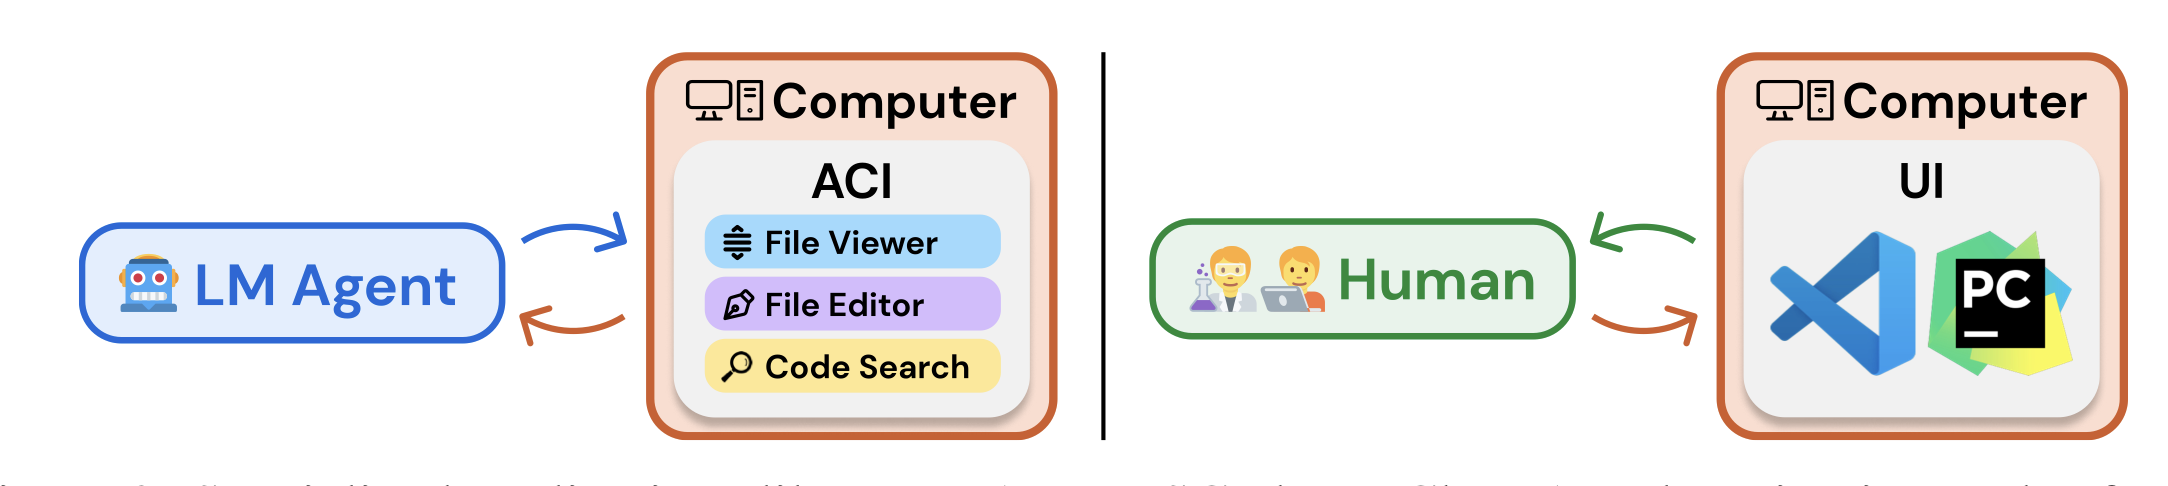
\includegraphics[width=\linewidth]{figures/swe.png}};
  \fill[ch13SweAgent] (185,252) rectangle (492,317);
  \node[text=blue!68!cyan!78!black,font=\fontsize{8.5}{10}\selectfont\bfseries] at (339,286) {语言模型智能体};
  \fill[ch13SweComputer] (771,76) rectangle (1035,126);
  \node[font=\fontsize{11}{13}\selectfont\bfseries] at (901,103) {计算机};
  \fill[ch13SweComputer] (1839,76) rectangle (2104,126);
  \node[font=\fontsize{11}{13}\selectfont\bfseries] at (1971,103) {计算机};
  \fill[ch13SweViewer] (758,225) rectangle (989,260);
  \node[font=\fontsize{8.8}{10}\selectfont\bfseries] at (873,244) {文件查看器};
  \fill[ch13SweEditor] (758,287) rectangle (989,324);
  \node[font=\fontsize{8.8}{10}\selectfont\bfseries] at (873,306) {文件编辑器};
  \fill[ch13SweSearch] (758,348) rectangle (989,387);
  \node[font=\fontsize{8.8}{10}\selectfont\bfseries] at (873,368) {代码搜索};
  \fill[ch13SweHuman] (1332,252) rectangle (1544,310);
  \node[text=green!45!black,font=\fontsize{12}{14}\selectfont\bfseries] at (1438,282) {人类};
\end{tikzpicture}
\endgroup

    \caption{用于软件工程的 SWE-Agent \citep{yang2024swe}}\label{fig:swe}
  \end{center}
\end{figure}

MLGym \citep{nathani2025mlgym} 沿用了广受欢迎的 Gym 强化学习框架 \citep{brockman2016openai}。Gym 在环境与智能体之间提供标准化接口。它于 2016 年推出，加速了强化学习算法的开发，推动了这一领域的进步。MLGym 还进一步借鉴了 SWE-agent，例如其文件编辑能力，展示了如何将科学发现过程建模为一个交互过程。研究讨论的应用覆盖数据科学、博弈论、计算机视觉、强化学习和自然语言处理等领域，并报告了使用商业大语言模型开展的实验，包括 OpenAI、Meta、Google 和 Anthropic 的模型。

包括研究助手和编程助手在内，大多数基于大语言模型的助手都依赖预先定义的工具，这限制了它们的自主性与可扩展性。Toolmaker \citep{wolflein2025llm} 通过让智能体直接根据科学论文及其代码仓库创建新工具，来应对这一局限。给定任务描述和 GitHub URL，它会安装依赖、配置可复现的 Docker 环境，并通过迭代的自我纠正和错误诊断，实现可用的 Python 工具。
该系统在 TM-Bench 上接受了评估。这个基准测试同样由 \citet{wolflein2025llm} 提出，包含医疗、生物学和人工智能领域的 15 项现实科学任务。Toolmaker 的任务成功率达到 80\%。其闭环设计使智能体不仅能够使用工具，还能够自主构建新工具，向能够自我扩展的研究助手与适应性科学工作流程迈进了一步。

Agent Laboratory 和 Toolmaker 等系统侧重于单个智能体的能力，而 The Agent Company~\citep{xu2024theagentcompany} 提供了一个综合基准测试，用于评估大语言模型智能体在接近真实工作的环境中的表现。它模拟一家小型软件公司，要求智能体使用浏览器、终端和通信平台等标准数字工具，完成从软件开发、项目管理到财务和人力资源等专业任务。

这一基准测试包含 175 项任务，旨在考察多步推理、工具使用，以及与大语言模型驱动的模拟同事协作的能力。每项任务都划分为若干检查点，用于衡量完全完成与部分完成的情况。使用包括 GPT-4o、Claude、Gemini 和 Llama 在内的 12 个基础模型开展的实验表明，即使是当前最强的系统，也只能自主完成约 30\% 的任务。失败往往源于通信、长程规划以及在复杂用户界面中导航等方面的不足。

The Agent Company 引入了一个可复现、自托管、映射现代工作场所的环境，为评估智能体大语言模型的成熟度提供了关键压力测试。它既凸显了当前系统的快速进展，也揭示了持续存在的局限，说明数字工作自动化已经触手可及，而真正的自主协作仍是一个重要的研究前沿。

\section{结语}

本章展示了智能体大语言模型如何作为助手，与现实世界交互。助手超越了被动问答，在对话、飞行运行、医疗、教育和科学研究等领域主动开展协作。它们进行规划、检索信息、调用工具、反思结果，并随着时间的推移调整自身行为。因此，智能体大语言模型使语言模型的角色从孤立的推理引擎，转变为更广泛的社会技术系统（socio-technical system）的参与者。

\paragraph{领域敏感性与风险}
并非所有助手都在相同约束下运行。医疗和航空等高风险领域要求对安全性、鲁棒性、透明性与公平性提供有力保障，也受到欧盟《人工智能法案》等监管框架的影响。在这些场景中，智能体设计越来越依赖检索、规划、验证与人类监督，而非端到端生成。学术研究也反映了这些关切，越来越强调将评估、偏见分析和可解释性作为首要设计目标，在设计之初就纳入考虑。

\paragraph{实践建议}
构建助手时，锚定（grounding，即在现实世界中评估）十分重要。应采用这样的架构：让智能体检索证据、说明行动理由，并在不确定时将决定交给人类，即让人类参与其中。将工具视为具有明确契约和失效模式的模块化组件。记录决策、计划与中间状态，以支持调试和审计。在高风险领域，我们建议在设计中考虑平稳降级（graceful degradation）；与自信地犯错相比，智能体请求澄清或选择不作答更为可取。

\paragraph{展望}
智能体助手的未来，在于更紧密地整合推理、学习与控制。要继续取得进展，需要更丰富的认知结构、从交互中持续适应，以及对安全与伦理提供更有力的保障。这些目标直接关系到可解释性与透明性方面的进展。在后续章节，尤其是机制可解释性一章（第~\ref{chap:mi}~章），我们将回到旨在打开黑箱的技术，更好地理解智能体大语言模型如何在内部表示目标、计划与决策。

\bibliographystyle{plainnat}
\bibliography{agenticbook,refs,case,synthetic}
